\documentclass[a4paper]{article}

\usepackage[english]{babel}
\usepackage[utf8]{inputenc}
\usepackage{amsmath}
\DeclareMathOperator*{\argmax}{argmax}
\usepackage{graphicx}
\usepackage[colorinlistoftodos]{todonotes}
\usepackage[nottoc]{tocbibind} % include references in contents page
\usepackage{color,soul} % for highlighting
%\usepackage[document]{ragged2e}
\usepackage[toc,page]{appendix} %appendix

\usepackage{listings}
\usepackage[most]{tcolorbox}
\usepackage{inconsolata}

\newtcblisting[auto counter]{sexylisting}[2][]{sharp corners, 
	fonttitle=\bfseries, colframe=gray, listing only, 
	listing options={basicstyle=\ttfamily,language=Python}, 
	title=Listing \thetcbcounter: #2, #1, top=0pt, bottom=0pt, boxsep=0pt, left=0pt}

\begin{document}

\begin{titlepage}
	\begin{center}
		
		
\includegraphics[width=0.8\textwidth]{NTU.png}
		\vspace{2cm}
		
		\huge
		
		\textbf{Pricing problems with \\Thompson Sampling}
		
		\vspace{1cm}
		\Large
		Lee Wai Leong Samuel
		
		\vspace{2cm}
		\Large
		Nanyang Technological University\\
		Division of Mathematical Sciences\\
		3 May 2019
		
		\vfill
		
		Final Year Project\\
		Supervisor: Dr. Yan Zhenzhen
		
		\vspace{0.8cm}
		
	\end{center}
\end{titlepage}
%\renewcommand{\baselinestretch}{1.5}
\begin{center}
	\large
	\textbf{Acknowledgements}
	\vspace{1cm}
\end{center}	
\large
%\renewcommand{\baselinestretch}{1.5}
My heartfelt thanks and gratitude go to Dr. Yan Zhenzhen for her patience and guidance throughout the project. There were times when I felt lost and was on the verge of giving up but she has been extremely understanding and encouraging. I have learned and grown tremendously both technically and personally from her knowledge and enthusiasm on this topic. It has been a great privilege to have her as my thesis supervisor.

\pagebreak
\begin{center}
%	\renewcommand{\baselinestretch}{1.5}
	\large
	\textbf{Abstract}
	\vspace{1cm}
\end{center}	
	\large
	In 1933, William R. Thompson proposed an algorithm known as Thompson sampling in order to maximise culmulative payoff in a multi-armed bandit (MAB) problem. MAB problems have been frequently used to model real-life decision making scenarios. This paper explores the extension of Thompson sampling to other problems beyond the MAB setting. More specifically, Thompson sampling is applied to product sales using data from a real dataset in a dynamic pricing setting as part of the multi-product pricing problem. 

\pagebreak
\large
%\renewcommand{\baselinestretch}{1.5}
\tableofcontents



\pagebreak
\section{Introduction}
\subsection{Background information}
E-commerce refers to the activity of buying or selling of products on online services or over the Internet. With sales reaching 10\% of total global sales, there is little doubt that e-commerce is a very popular online activity \cite{nano3}. It is even expected to continue growing to 15\% in 2020 which has led to many firms setting up their own e-commerce portals or through other e-commerce giants such as Amazon or Alibaba in order to take advantage of the proliferation of the Internet. E-commerce holds many advantages over traditional brick-and-motar stores. They do not have to pay rent, are not physically constrained by shelf space and they can easily change prices. They are also not restricted to operational hours since anyone with an Internet-capable device can browse their catalogue from virtually anywhere, anytime. Moreover, it is easier for them to study their customers' purchasing patterns such as their browsing history, products bought in the past and popular items in general. Using this information, sellers are able to offer a more personalised experience to their customers in order to help with customer retention and attraction.
\newline
\newline
As mentioned, it is much easier for e-commerce firms to change prices. A natural question that arises would be: how should products be appropriately priced so as to maximise revenue? If products are priced either too high or low, it may hurt the firm's image and cause poor customer experience which would lead to low revenue. Furthermore, most e-commerce firms have a large catalogue of products which further complicates price changes. This problem has been frequently modelled as the multi-armed bandit (MAB) problem where there are several possible price points to choose from. It involves making a decision at every time period with the objective of maximising reward at the end of all time periods. Each decision corresponds to a set of possible prices while reward corresponds to revenue at the end of the selling season. Behind each decision lies a demand function reflecting customers' purchasing behaviour which is not directly observable. The seller then has to balance between learning each demand function to increase revenue in the long term (exploring) and earning revenue in the short term (exploiting). This is known as the exploration-exploitation trade-off. Regret is defined as the difference in expected revenue of an algorithm compared to the expected revenue of the ideal case when the demand functions are known at the beginning. Any solution to the MAB problem seeks to minimise regret. Once the seller knows the best decision, they may then exploit it for the rest of the selling season in order to maximise revenue. In practice, the parameters of each demand function are not known and have to be learned over time. Brick-and-motar stores do not face this problem since they do not frequently change prices due to high costs \cite{anderson} and hence, practice static pricing. Static pricing does not harness the advantages of going online and is too naive to simulate the true demand function.  In addition, brick-and-motar stores do not have a large catalogue of products which simplifies the pricing of products.
\newline
\newline
In contrast to static pricing, dynamic pricing involves a seller regularly adjusting the prices of products in order to obtain information about the products' demand, and then exploiting this information in order to maximise revenue. The MAB problem described previously is an example of dynamic pricing. By manipulating prices, firms are able to respond to competitors and learn more about customer behaviour. Dynamic pricing solutions typically follow these steps: propose a demand model as a function of price, estimate the model's parameters from historical data, optimise revenue to obtain new prices using the learned demand model and then implementing the new prices and repeating.
\newline
\newline
One way to implement price changes would be to model them as sales promotions. Sales promotions are also frequently implemented for clearing excessive stock, attracting customers and increasing short-term revenue. Some common examples of promotions include percentage discounts (X\% off), flat amount discounts (\$X dollars off), BOGO (Buy one get one at X\% off) and multi-buys (2 for the price of 1). Percentage discounts are probably the most frequently implemented sales promotion in practice as they are simple to understand and implement. In addition to these promotions that are targeted at changing prices, there are also other types of indirect promotions such as loyalty programs, contests, coupons and giveaways. Loyalty programs involve offering customers some form of bonus or reward for purchasing their products. Examples of loyalty programs are reward cards or points systems. The customer accumulates rewards or points with every purchase and this may encourage them to make repeat purchases to build customer loyalty. Sending virtual coupons to customers will make the promotion seem more exclusive and personalised and may encourage spending too. Coupons are also a great way to win over dissatisfied customers. With the Internet being easily accessible these days, many firms hold contests online on social media platforms. The firm only has to give away one or a few products but in return, their profile may be raised by increasing exposure to potential customers.

\subsection{Motivation}
To provide additional motivation for this problem, we have a real dataset from an e-commerce firm based in China. The dataset consists of sales data of 66 products (children's books) sold over a period of 11 days without any changes in price while under some sales promotion. There are 4716 rows and 23 columns. Each row represents a product in an order that was placed while each column represents a feature of each order such as order ID, order date, user ID, goods ID, price and quantity.
\newline
\newline
If we analyse the summary statistics of columns that make sense i.e. columns that are not IDs or time and date, we obtain the following:
\begin{figure}[h]
	\centering
	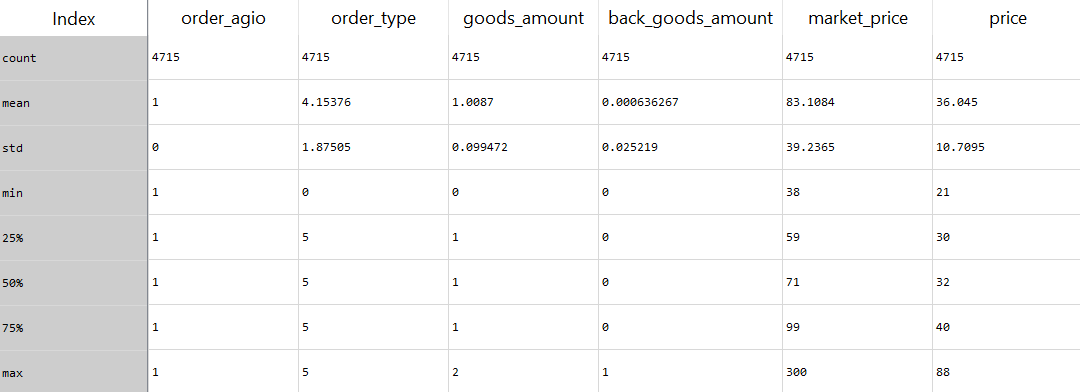
\includegraphics[width=1.1\textwidth]{data1.png}
	\caption{\label{fig:data1}Summary statistics of columns}
\end{figure}
\begin{figure}[h]
	\centering
	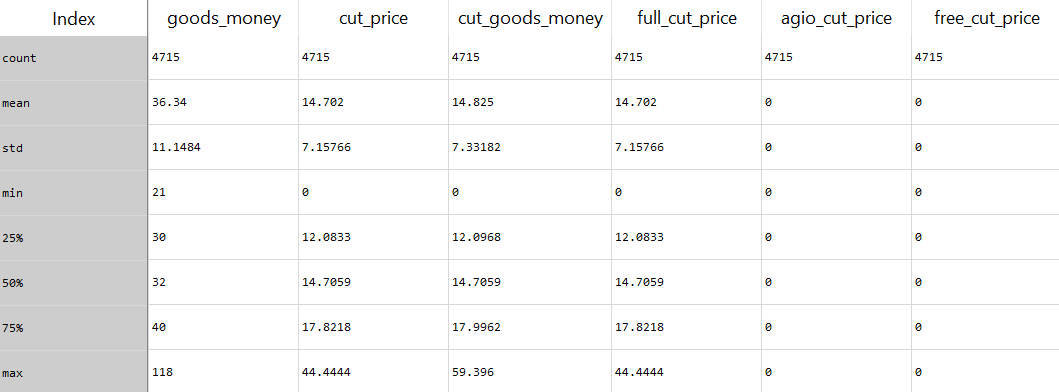
\includegraphics[width=1.05\textwidth]{data2.png}
	\caption{\label{fig:data2}Summary statistics continued}
\end{figure}
\newline
\newline
Let us take a look at some columns that are more interesting. In Figure \ref{fig:data1}, $market\_price$ is the market price of products while $price$ is the selling price of products. At all levels (min, mean, median, max etc), $price$ is lower than $market\_price$ which suggests that the seller might be trying to clear inventory by possibly selling the products at a loss. $goods\_money$ is the amount a customer paid for a product and it also takes into account the quantities of products purchased. Its max value is 118 because there were customers that bought 2 quantities of a same product that costs 59. All products that cost greater than 58 were bought only once in each order and thus, their $goods\_money$ values are less than 2 * 59 = 118. Even the most expensive product that costs 88 was only bought once. Similarly, $cut\_price$ is the amount a customer can save on a product due to all ongoing sales promotions (on top of lowering prices to $price$) and $cut\_goods\_money$ is $cut\_price$ with quantities ordered factored in.
\newline
\newline
The last 3 columns $full\_cut\_price$, $agio\_cut\_price$ and $free\_cut\_price$ in Figure \ref{fig:data2} correspond to amounts a customer can save on a product due to each promotion. $full\_cut\_price$ refers to the amount saved due to a full-cut promotion. In a full-cut promotion, there is usually a pre-determined amount called a threshold. For each time an order satisfies the threshold amount, it would be eligible for a flat amount of discount. For example, Calvin Klein recently had the promotion "For every \$100 spent, enjoy \$40 off" on their website \cite{CK}. This means that customers are encouraged to spend more since they may also potentially save more. $agio\_cut\_price$ refers to the amount saved due to a percentage discount promotion while $free\_cut\_price$ refers to the amount saved due to a "Buy X get Y free" promotion. Since the last two columns are 0, this means that the only ongoing sales promotion in the dataset is the full-cut promotion. This is further substantiated by the fact that the $cut\_price$ column has the same values as the $full\_cut\_price$ column which means the amount saved for each product due to promotions is the same as the amount saved due to a full-cut promotion. Lastly, we can verify the existence of a full-cut promotion by testing several threshold values through trial and error. 
\newline
\newline
If $X$ is trialed as the threshold value, orders can be categorised into groups of different multiples of $X$. The first group would consist of orders ranging from \$0 to \$($X$-1) and the second group would range from \$$X$ to \$2$X$-1 and so on. The mean discount for each group can then be calculated. If $X$ is the threshold value, the mean discount for the first group should be 0 as all orders in that group should not have fulfilled the minimum amount. Likewise, the mean discount for subsequent groups should be multiples of the discount. Plotting the mean discounts for each group should reveal a linear relationship.
\begin{figure}[h]
	\centering
	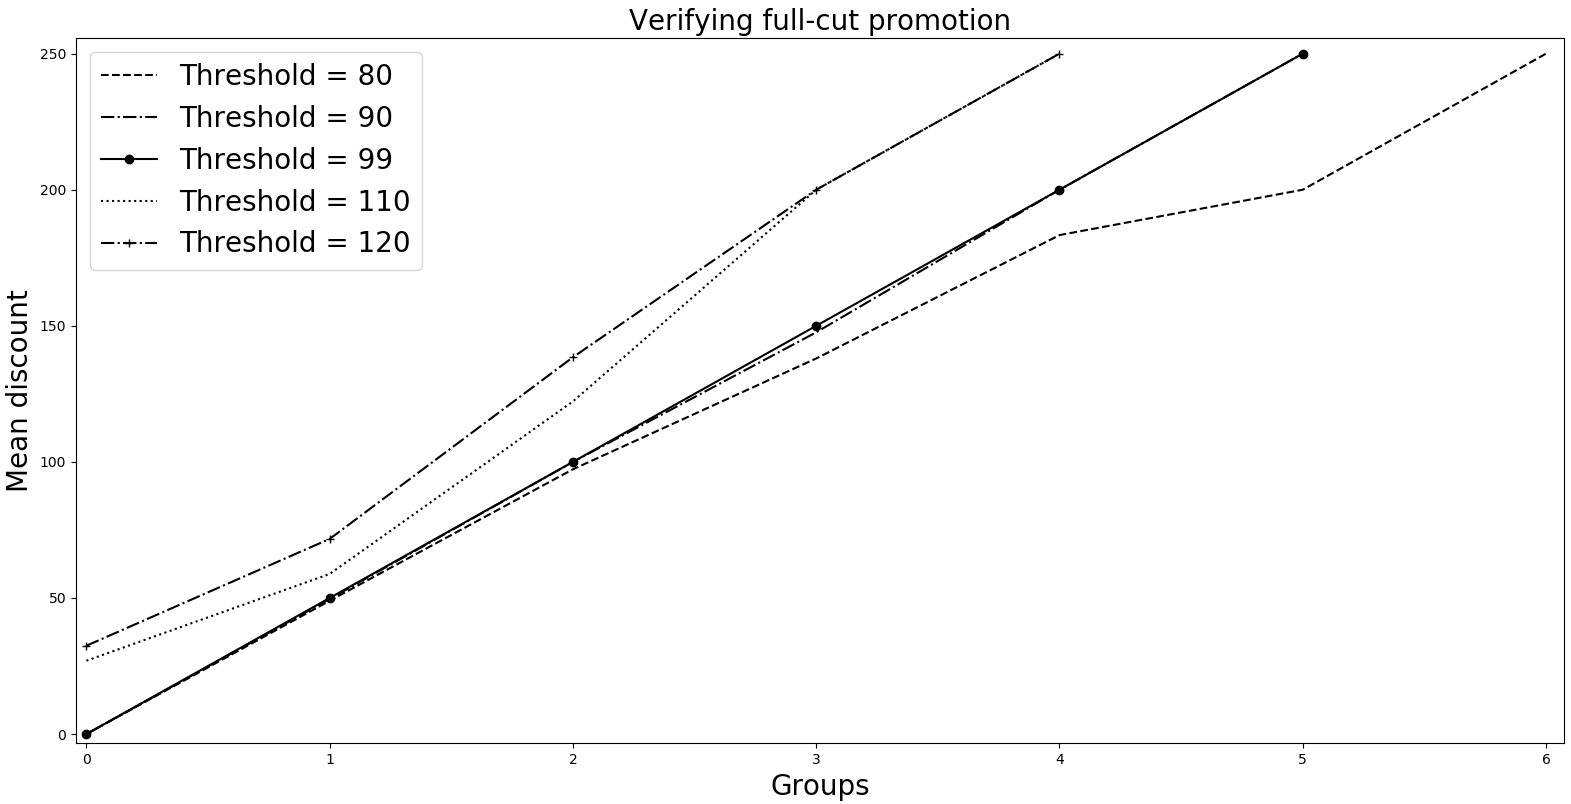
\includegraphics[width=1.05\textwidth]{threshold.png}
	\caption{\label{fig:threshold}Plotting mean discounts for each group}
\end{figure}
\newline
\newline
For this data set, multiple values of $X$ (80, 90, 99, 110, 120) were tested and the mean discounts were plotted in Figure \ref{fig:threshold}. For $X = 80, 110$ and $120$, the gradients are not constant over each group. This suggests that some groups contain orders that qualify for different discounts from the rest. On the other hand, the plots of $X = 90$ and $X = 99$ indicate a strong linear relationship. However, at $Groups = 3$, the plot of $X = 90$ is not as linear as $X=99$. Thus, it is likely that the true threshold value of this data set is 99.
\newline
\newline
In the dataset, the last two columns ($agio\_cut\_price$ and $free\_cut\_price$) in Figure \ref{fig:data2} corresponding to different sales promotions were also included even though they were not actively implemented in this selling season. This suggests that sales promotions like these are frequently implemented during different selling seasons and thus warranted a permanent slot in the dataset. We may infer that sales promotions are crucial to the performance of a seller's business and we should investigate them further.
\newline
\newline
\newline
This dataset drives the main motivation of this paper. Here, we can see that the seller has designed several types of sales promotions. In this specific selling season, they are trying to implement full-cut sales promotions in order to increase product sales. In this paper, we will explore dynamic pricing modelled as discounts in sales promotions for every time period. More specifically, we are interested in applying the Thompson sampling algorithm to solve the dynamic pricing problem. We first compare the results of Thompson sampling to other popular algorithms in a MAB problem before moving to a more general dynamic pricing setting where there are infinite arms. Specifically, we will implement a variant of Thompson sampling proposed by Ganti, Sustik, Tran \& Seaman (2018). While many other efficient algorithms exist to solve dynamic pricing problems, Thompson sampling was chosen as it has been shown to be highly competitive with promising performance \cite{thomp}. 


%\newpage
\section{Literature review}
In order to study sales promotions, the multi-product pricing problem should first be investigated as it is a more fundamental problem of dynamic pricing problems. In this area, work has been done in the cases of known demand function and unknown demand function. In the former case, the dynamic pricing problem is typically modelled as the multi-armed bandit (MAB) problem and is solved by well-known methods such as the upper confidence bound (UCB) algorithm. Bubeck \& Cesa-Bianchi (2012) summarised this problem without resource constraints in their paper. Badanidiyuru et al. (2013) further improved on this approach by adapting the UCB algorithm to a MAB problem with resource constraints as such constraints cannot be easily modelled in the typical MAB problem. This was achieved by maintaining a vector of costs and adjusting it by combining confidence bounds and multiplicative updates. 
\newline
\newline
In the latter case of unknown demand function, Aviv \& Pazgal (2005) used a certainty-equivalent heuristic to obtain an approximate pricing solution in a partially observed Markov decision process (POMDP) framework. Both Araman \& Caldentey (2009) and Farias \& Van Roy (2010) extended on this approach by proposing more sophisticated approximate dynamic programming heuristics. Araman \& Caldentey (2009) used a sequence of models with varying levels of complexity to model the demand in which the underlying process followed a Poisson distribution, and then proposed a set of algorithms that efficiently approximated the solution. Similarly, Farias \& Van Roy (2010) also used a Poisson distribution for their model but with a different heuristic approach which they called \textit{decay balancing.} Broder \& Rusmevichientong (2012) used maximum likelihood estimation to obtain pricing policies under a general parametric choice model and also when the family of demand functions satisfied a ``well-separated" condition. 
%\newline
%\newline

%\newpage
\section{Description of approaches}
\label{sec:approach}
The first approach would be to use the classical Thompson sampling algorithm in a MAB problem where each price vector represents an arm. In this approach, there is a finite number of price vectors and this falls under discrete pricing. The goal is to learn the demand distribution and expected payout of each price vector so as to maximize revenue over time. We consider two cases in this approach: when the demand function is a multinomial-logit (MNL) model and when it is a constant price elasticity model. We chose these two demand models because they are frequently used in studies and we do not consider any forms of constraints. The performance of Thompson sampling is then compared to other commonly used algorithms for the MAB problem.
\newline
\newline
The second approach would be to use Thompson sampling in a dynamic pricing algorithm. More specifically, we apply the Thompson Sampling algorithm for dynamic pricing with continuous prices proposed by Ganti, Sustik, Tran \& Seaman (2018). Their algorithm works as follows: a Bayesian prior is initialised on unknown parameters using historical data. The posterior is obtained via Bayes rule and a sample is taken from this posterior as an estimate of parameters. A new set of prices (likely to be different from the previous time period) is obtained by maximising a reward function with the sampled parameters. This process will continue until the end of all time periods. In this approach, there is usually a larger set (possibly infinite) of price vectors in contrast to the MAB setting which only has fixed price vectors. The goal is to learn the distribution of the price elasticity of each product in order to maximise revenue and not the distribution under each price vector. We will also consider two cases in this approach: when the demand function is a non-stationary modified constant elasticity function which will be explained in greater detail later and a stationary regular constant elasticity function. In each of these cases, we will further impose inventory constraints and explore the performance. Lastly, the performance of this specific Thompson sampling algorithm in this approach will also be compared to the static pricing strategy i.e. no dynamic pricing algorithm is implemented.

%\newpage
\section{First approach: Discrete prices}
In this section, we will consider discrete sets of prices i.e. finite sets of prices. This corresponds to having a finite number of arms in a typical MAB problem. We implement the classical Thompson sampling algorithm to solve a MAB problem under different demand functions, namely the MNL model and the constant price elasticity model. We then compare the performance of the algorithm to the best possible outcome in each demand function before comparing with other well known algorithms. Both of these demand functions were chosen in order to observe how Thompson sampling performs under different conditions. Moreover, the constant price elasticity model is closely related to our second approach in section 5.

\subsection{Multinomial-Logit model}
In a MNL model, the logistic function is generalised to multi-class problems with more than two possible outcomes. In this specific setting, each class represents the probability of a customer purchasing a specific product. It thus assumes that every customer's purchasing behaviour is homogeneous.

\subsubsection{Data generation}
The only information we use from the dataset in this subsection is the set of prices of all products, which will represent one arm of the MAB problem. Two other price vectors were created by adding and subtracting $10\%$ to the original price vector. Together, we may identify the 3 price vectors as lower price vector, middle price vector and higher price vector where the lower price vector is 10\% less than the middle price vector. The method described below was used to create simulation data.
\newline
\newline
For each price vector $k$, 1 data point was created using the MNL formula below and it will represent the mean of the true demand under that price vector
\[X_{i,k} = \frac{e^{V_i - p_{i,k}}}{\sum_{j=0}^{N}e^{V_j - p_{j,k}}} \]
where $V_i$ represents the customer's utility of product $i$ and $p_{i,k}$ is the price of product $i$ under price vector $k$. Thus, $X_{i,k}$ is the mean of the true demand for product $i$ under price vector $k$.  In other words, $X_{i,k}$ is the probability of a customer purchasing product $i$ under price vector $k$. In the denominator, $j=0$ represents the option where the customer chooses not to buy anything and $N$ refers to the total number of products.
\newline
\newline
As there are now 3 price vectors, the utility vector $V$ can be created by randomly sampling from a 5\% neighbourhood of $\hat{p}$ where $\hat{p}=\sum_{k=1}^{3}p_k$. $V_0$ is randomly sampled from the interval $(0,5).$
\newline
\newline
With the $V$ and $p$ vectors defined, the theoretical $X_i$ corresponding to each price vector $k$ can be created and they will represent the true demand. In the long run, the expected value of all data points for each price vector should be equal to the theoretical $X_i$.
\newline
\newline
For each price vector, 20 data points were created as historical data in order to obtain our prior distribution. In order to ensure that the expected value of all data points was equal to the theoretical $X_i$, 10 epsilon vectors were created and the data points were obtained by adding and subtracting the epsilon vector from the theoretical $X_i$. This process was repeated for the other two price vectors as well. In total, there were 60 data points created with each price vector having 20 data points to serve as historical data.

\subsubsection{Implementation of classical TS}
In this approach, the objective was to learn the true demand function under each price vector. It was assumed that the true demand functions followed normal distributions. The prior distribution for each price vector was then estimated from the 20 data points generated earlier using maximum likelihood estimation. 
\newline
\newline
For iterations $t = 1,...,T$, the following process was done:
\begin{enumerate}
	\item A random sample was taken from each price vector's prior distribution.
	\item The estimated revenue under each price vector was calculated by multiplying the random sample and the price vector since each random sample represents the estimated demand under that price vector.
	\item The price vector with the highest estimated revenue was chosen as the selected arm for this iteration.
	\item The selected arm was pulled. The observed demand would be that price vector's theoretical $X_i$ i.e. if arm $k$ was pulled, the observed demand would be $X_{i,k}$.
	\item The observed revenue was calculated by multiplying the observed demand with the price vector and also accumulated over all iterations.
	\item The observed demand was added as an observation to the selected arm's $H_{t-1}$ data points where $H_{t-1}$ is the number of data points under that price vector in the previous iteration.
	\item The prior distribution of that price vector was re-estimated with the $H_{t-1} + 1$ data points using maximum likelihood estimation.
\end{enumerate}
%\newline
%\newline
The number of times each price vector was selected was recorded. The price vector that was selected the most often would then be the arm with the highest revenue.
\newline
\newline
In order to validate that the chosen arm in the above process was the correct arm, a simple check was conducted for each arm. In each check, the same arm was chosen in every iteration and the observed revenue was cumulated. The arm with the greatest cumulated revenue would then be the theoretically correct arm. The average result of 10 initialisations of this approach over 1000 iterations is shown in Figure \ref{fig:one}. $T$ was set to be 1000 in order for us to observe any long term effects.
\newline
\newline
The dashed, dashed-dotted and dotted lines correspond to checks for each arm and they represent the true revenue under that arm. The solid line with circles represents the revenue under classical Thompson sampling and interestingly, it has the exact same values as the lower arm in every iteration which is why the lower arm cannot be seen. Since the lower arm has the highest cumulated revenue out of all three arms, it is the theoretically correct arm. This means that Thompson sampling had already correctly identified the best arm right from the beginning and was exploiting it in every iteration.
%\newpage
\begin{figure}[h]
	\centering
	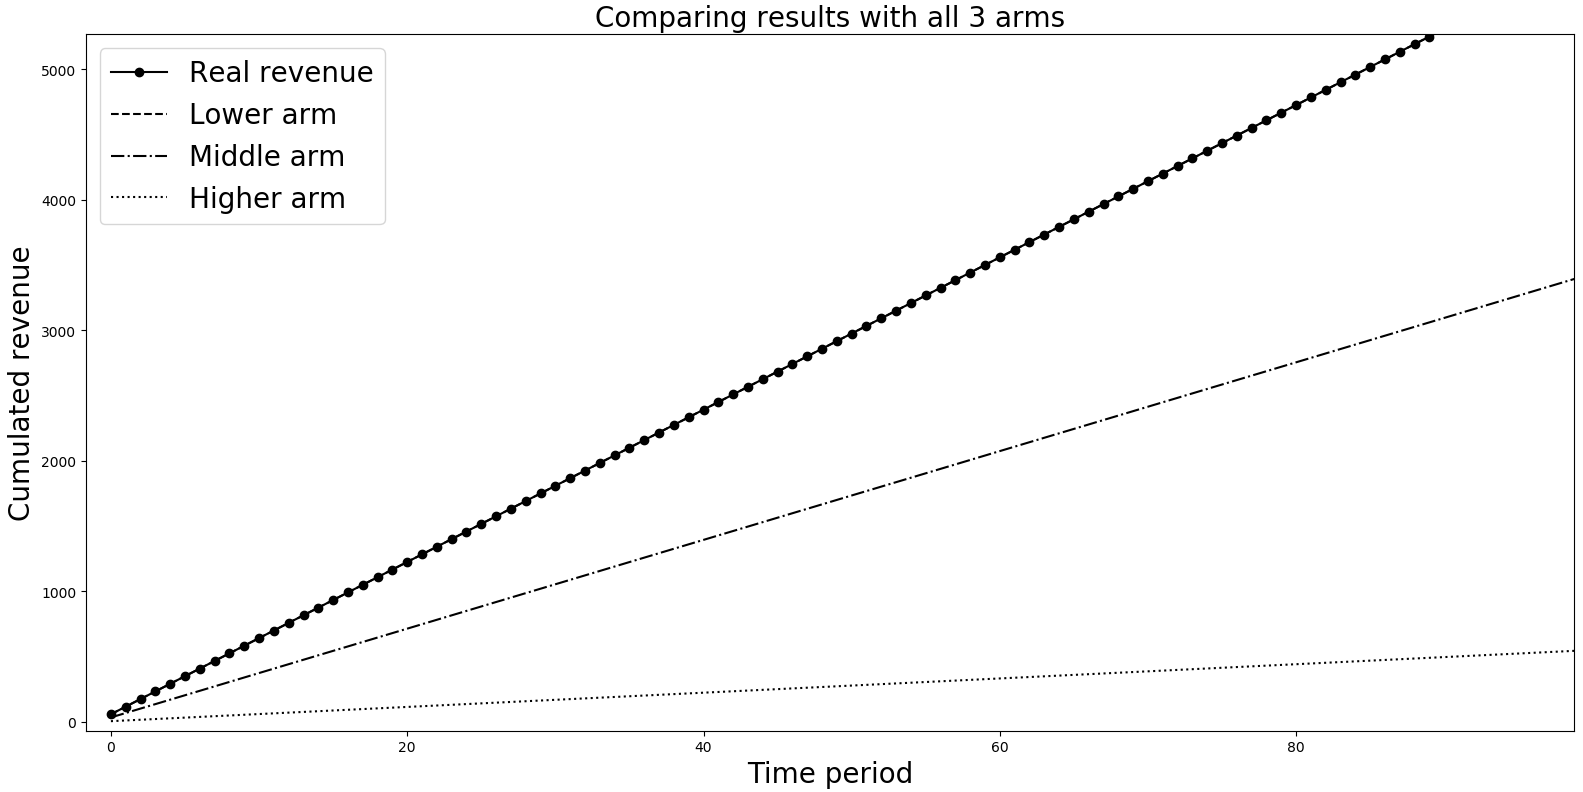
\includegraphics[width=1.03\textwidth]{Figure_1-2.png}
	\caption{\label{fig:one}Comparing revenue between all 3 arms and actual revenue (MNL model)}
\end{figure}

\subsubsection{Comparison with other algorithms}

As mentioned earlier, the MAB problem is not new and many algorithms have been developed to solve it. Here, we compare the performance of Thompson sampling to other well-established algorithms in the same setting as the previous subsection. The algorithms we'll compare to are:
\begin{enumerate}
	\item Upper Confidence Bound - UCB1
	\item Upper Confidence Bound Tuned - UCB1-Tuned
	\item Epsilon-greedy algorithm
	\item Epsilon-greedy with optimistic initialisation
	\item Epsilon-greedy with decay	
\end{enumerate}
%\newline
%\newline
According to Figure \ref{fig:two}, the performance of the algorithms are all very similar in the beginning. The epsilon-greedy algorithm even manages to match Thompson sampling until the 7th time period. However, if we observe the results at the end of the horizon in Figure \ref{fig:three}, the epsilon-greedy algorithms perform significantly poorer than TS. Unsurprisingly, greedy algorithms do not work well in most situations since they exploit too much and explore too little. UCB algorithms have been widely considered to be good solutions to MAB problems since they have small regret. From this example, we see that Thompson sampling also outperforms them although to a smaller extent. This is probably because Thompson sampling assumes a prior distribution from historical data while UCB does not, and instead requires the pulling of every arm (including suboptimal ones) at least once in the beginning which contributes to increased regret.
\vfill
\begin{figure}[h]
	\centering
	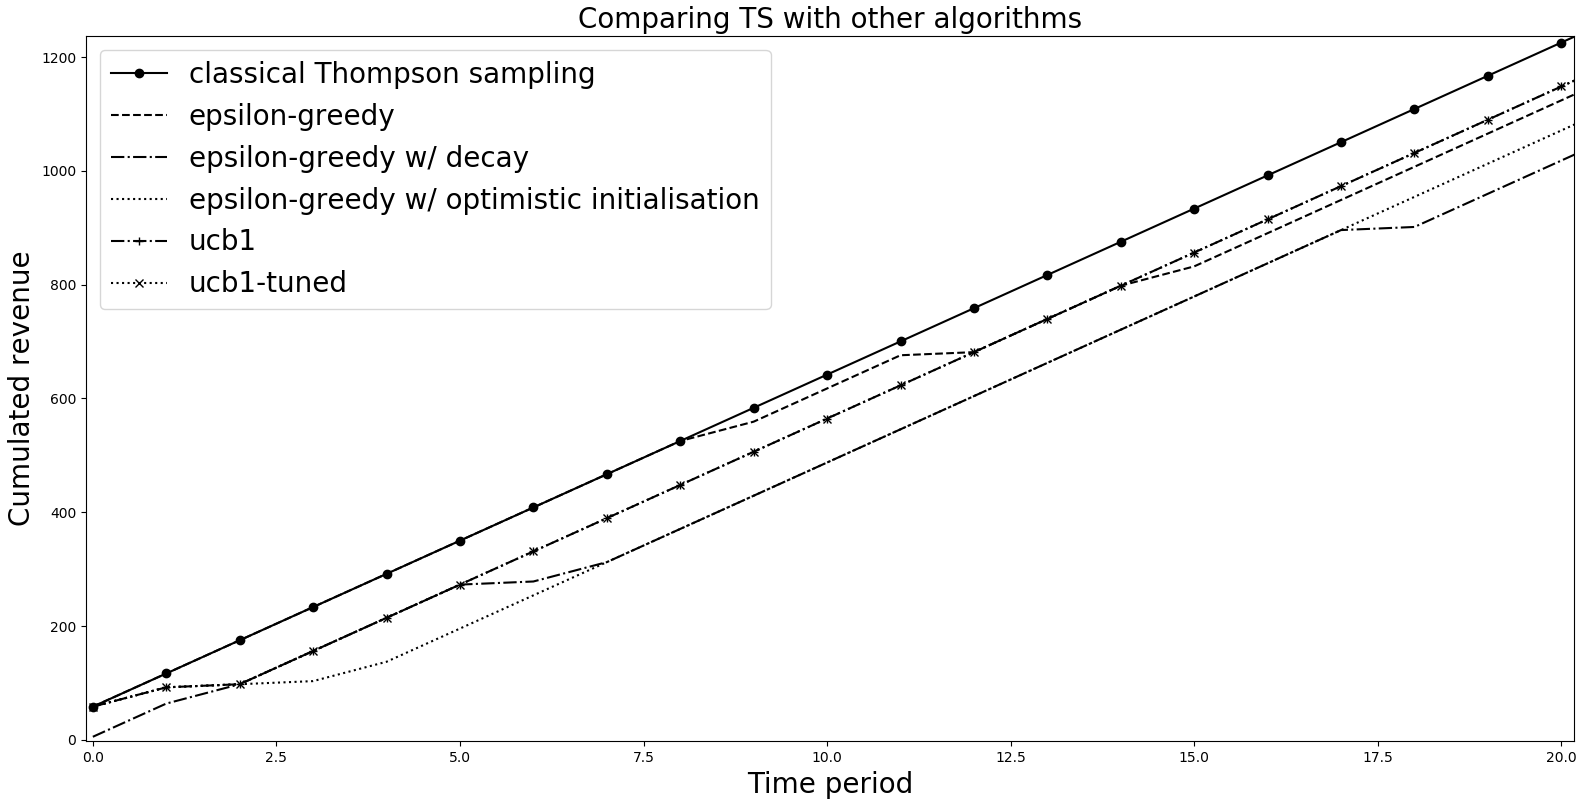
\includegraphics[width=1.03\textwidth]{Figure_1-3.png}
	\caption{\label{fig:two}Comparing revenue between all algorithms - first 20 time periods (MNL model)}
\end{figure}
\vfill
\begin{figure}[h]
	\centering
	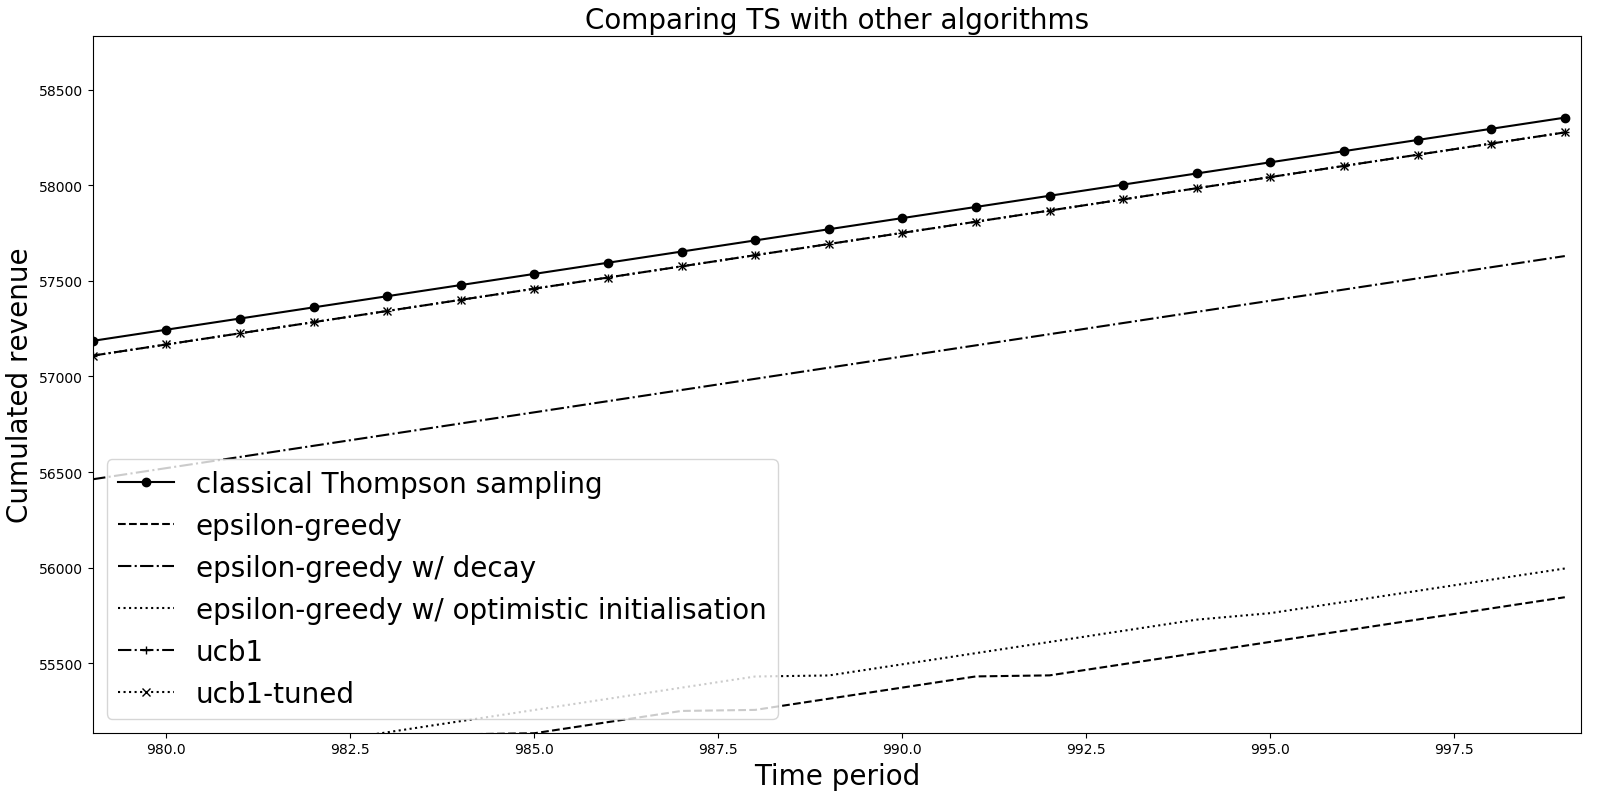
\includegraphics[width=1.03\textwidth]{Figure_1-4.png}
	\caption{\label{fig:three}Comparing revenue between all algorithms - last 20 time periods (MNL model)}
\end{figure}

\newpage


\newpage
\subsection{Constant price elasticity model}
In a constant price elasticity model, each product's elasticity of demand is taken into account. Elasticity of demand refers to the responsiveness of the quantity demanded of a good or service to a change in its price. Unlike the MNL model, the constant price elasticity model produces the absolute quantity of products sold and not the probability of products being purchased. Therefore, it is more concerned with market demand as a whole, rather than each individual customer's purchasing behaviour.

\subsubsection{Data generation}
The remaining subsections are very similar to the previous subsections under the MNL model and so we will skip most of the repeated work. Instead, we will point out where the main differences lie.
\newline
\newline
Similar to the previous subsection using the MNL model, we reuse the same 3 price vectors for $k = 1,2,3$. The demand function under the constant price elasticity model is given below. 
\[d_{i,k} = f_{i,0} \left(\frac{p_{i,k}}{p_{i,0}}\right)^{\gamma_{*,i}} \]
To recap, our dataset consisted of 11 days of data and we chose the first day to be set as the baseline demand $f_{i,0}$ since every product was sold at least once on the first day. This ensures that the starting point of the algorithm uses real data. $\gamma_{*,i}$ was randomly generated once to be some random vector where $\gamma_* \in [-3, -1]^{66}$ and fixed throughout the entire horizon. The middle price vector $p_{i,2}$ from the previous subsection, which is also the price from our dataset, was set as the baseline price $p_{i,0}.$ $d_{i,k}$ thus refers to the quantity demanded of product $i$ under price vector $k$.
\newline
\newline
Since we now have our theoretical demand $d_i$ corresponding to each price vector $k$, we can again create historical data in the same manner as before by creating epsilon vectors and then performing addition and subtraction. This would ensure that the means for our historical data for each price vector would be equal to the theoretical demand.

\subsubsection{Implementation of classical TS}
In this approach, the objective remains the same: to learn the true theoretical demand under each price vector. Again, we assumed that the true demands followed normal distributions and we wished to learn the parameters of the distributions. We initialised our prior distributions for each price vector on the historical data that we created through the method of maximum likelihood estimation.
\newline
\newline
The process is exactly the same as that described in section 4.1.2, bar step 4. In this setting, the observed demand would be $d_{i,k}$ depending on which price vector $k$ was chosen.
\vfill
\begin{figure}[h!]
	\centering
	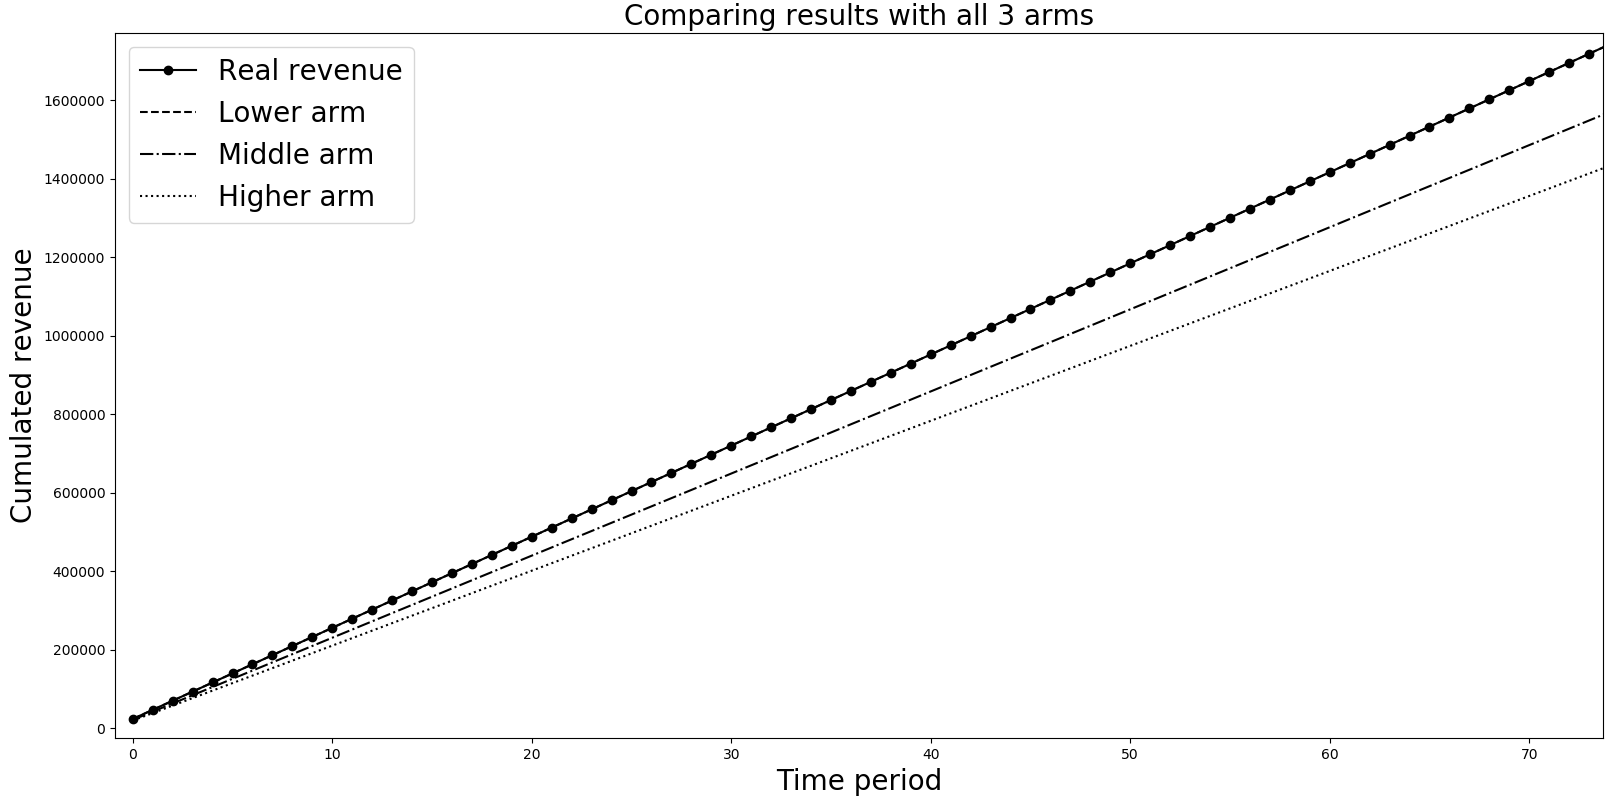
\includegraphics[width=1.03\textwidth]{7.png}
	\caption{\label{fig:7}Comparing revenue between all 3 arms and actual revenue (constant elasticity model)}
\end{figure}
\vfill

Similar to Figure 4, we again see that Thompson sampling had already correctly identified the best arm from the beginning and was exploiting it in every iteration in Figure 7.

\subsubsection{Comparison with other algorithms}
We again compare the performance of Thompson sampling to other well-established algorithms as in the previous subsection. From Figures 8 and 9, we see that the results are consistent with our previous observations. Thompson sampling and the UCB algorithms both outperform the greedy algorithms. However, the difference in cumulated revenue between Thompson sampling and UCB is much smaller under the constant price elasticity model. By the end of the horizon, Thompson sampling still outperforms the UCB algorithms.
\begin{figure}[h!]
	\centering
	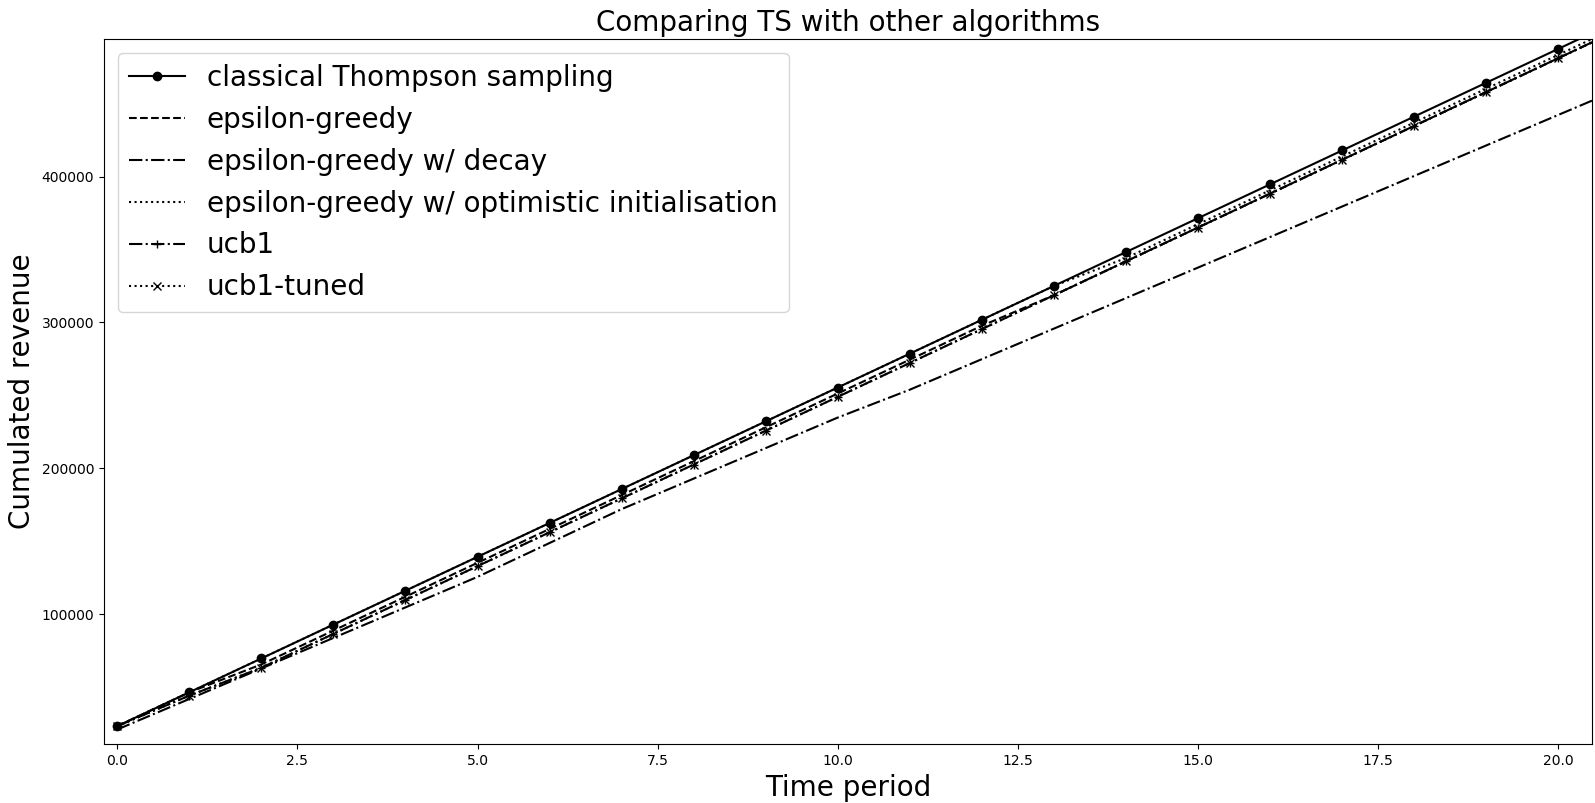
\includegraphics[width=1.03\textwidth]{5.png}
	\caption{\label{fig:5}Comparing revenue between all algorithms - first 20 time periods (constant elasticity model)}
\end{figure}
\begin{figure}[h!]
	\centering
	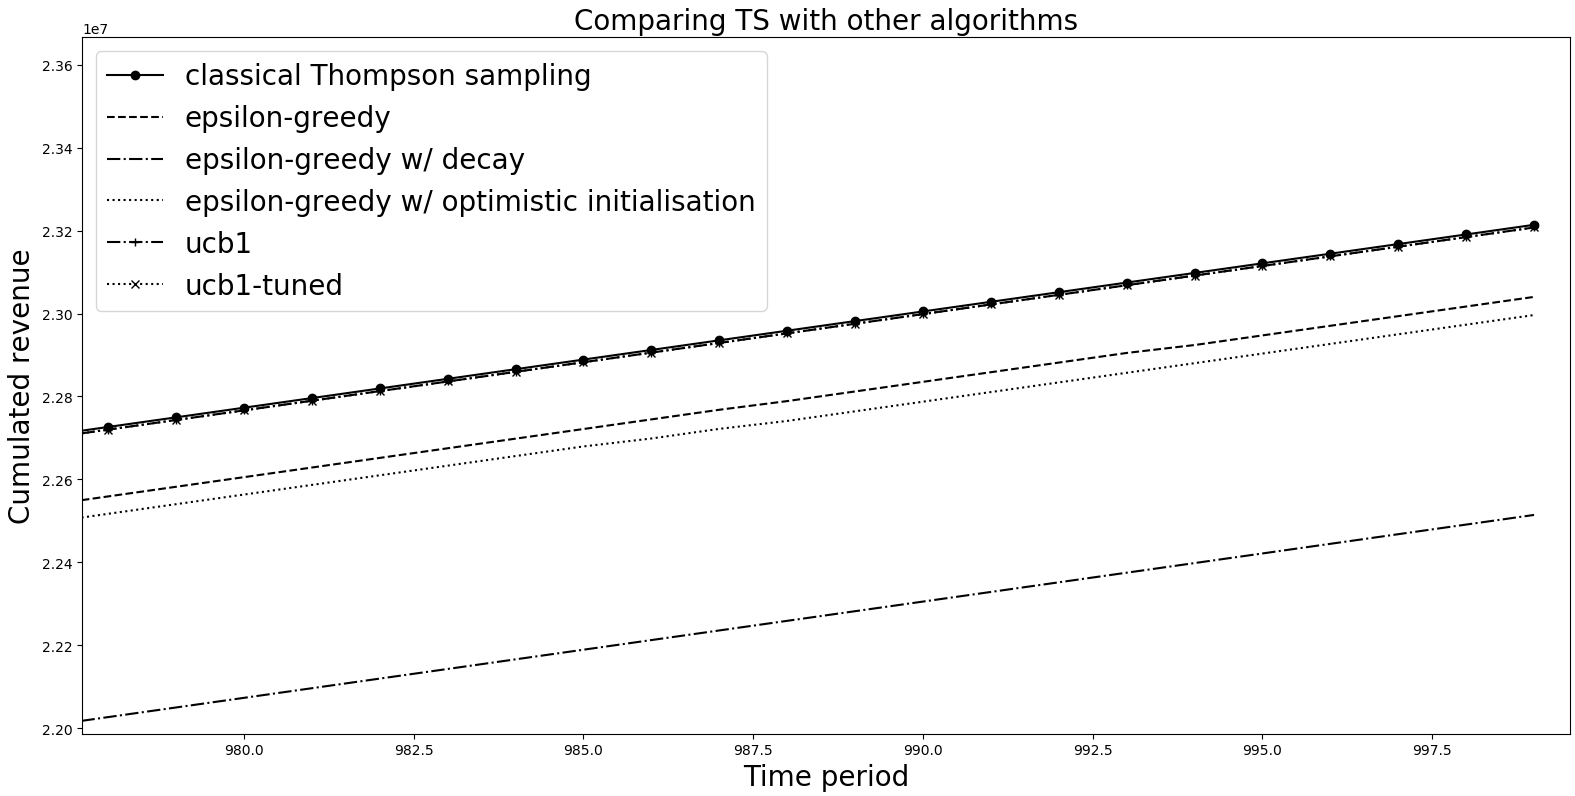
\includegraphics[width=1.03\textwidth]{6.png}
	\caption{\label{fig:6}Comparing revenue between all algorithms - last 20 time periods (constant elasticity model)}
\end{figure}
\newpage
\subsection{Conclusion of first approach}
In this section, we have seen that Thompson sampling is relatively robust as it worked well in two commonly used demand functions, namely the MNL model and the constant price elasticity model. It is worth noting that in both of these settings, we had reliable historical data since taking the mean of the data actually produced the true theoretical demand. Repeating the experiments with poor or no historical data (i.e. random initialisation of parameters) may yield interesting results in which other algorithms may possibly outperform Thompson sampling. Another possible extension would be to consider non-stationary demand functions as part of the non-stationary bandit problem.

\section{Second approach: Continuous prices}
In this approach, the objective is to learn the true elasticity values for each product. We implement the Thompson sampling algorithm for dynamic pricing proposed by Ganti, Sustik, Tran \& Seaman (2018). In their paper, they consider the demand function to be a modified constant elasticity model. The commonly used constant elasticity model is 
\[d_i(p_i) = f_i \left(\frac{p_i}{p_{i,0}}\right)^{\gamma_{*,i}} \tag{1} \] 
where $d_i(p_i)$ is the demand of item $i$ at price $p_{i}, f_i$ is the baseline demand at price $p_{i,0}$ for item $i$ and $\gamma_{*,i} < -1$ is the elasticity of item $i$. This is also the demand function that was implemented in section 4.2. Instead of this model, the authors proposed 
\[d_{i,t}(p_i) = f_{i,t} \left(\frac{p_i}{p_{i,t-1}}\right)^{\gamma_{*,i}} \tag{2}\]
which we will implement for this approach. Notice that the notation is slightly different from what we used in the previous section. This is because we only considered discrete price points i.e. finite sets of prices in section 4 and now we are considering continuous price points i.e. infinite sets of prices. $f_{i,t}$ is the demand forecast for item $i$ on day $t$ using observed demand for item $i$ at different price points on days $t = 1,..., t-1$. $f_{i,t}$ can be obtained using various models. Some suggested examples include time series models such as ARMA, ARIMA, AR(k) or non-time series models such as logistic regression or even a combination of models to form a new model. In our application, we used a simple AR(k) model as suggested by the authors.
\newline
\newline
This modified model has several advantages over the MNL model and the typical constant elasticity model. Firstly, the demand function in real world pricing systems is usually not stationary and the adaptations made can reflect this property by accounting for possible movements in the underlying demand function. Secondly, the MNL model assumes homogeneous customer behaviour i.e. every customer has the same purchasing behaviour. On the other hand, the constant elasticity model is an aggregate model i.e the model perceives the market as a whole and not as one customer. This may be more reflective of demand in a real world setting.
\newline
\newline
Also, we would like to emphasise on the definition of stationarity. We understand that in certain papers and literature, non-stationary demand functions may mean entirely different demand functions in different time periods or the products' elasticity may be a variable generated from different functions. In this paper, the difference between our stationary and non-stationary demand functions lies in its parameters. The non-stationary demand function has parameters ($f_{i,t}, p_{i,t-1}$) that change in each time period. However, both are still considered constant price elasticity models. 
\newline
\newline
In this section, we will compare the results of the dynamic pricing algorithm to a model with no dynamic pricing implemented, which we will call the constant price model. Static pricing is implemented instead i.e. prices are kept constant throughout the selling season. The comparison will be done in two settings - one with the stationary demand function in (1) and the other with non-stationary demand function in (2). For each of these settings, we further consider cases where inventory constraints are present and absent.
\newline
\newline
The dynamic pricing algorithm needs a prior distribution $\Pi_0(\gamma_*)$ which is assumed to be a normal distribution for the elasticity and an estimate for the noise variance $\sigma^2$. The authors suggest using prior elasticity estimates from historical data as the mean $\mu_0$ of the prior distribution and $\Sigma_0 = cI$ for some constant c as the covariance matrix. Similarly, sample standard deviation of observed revenue from historical data can be used to estimate $\sigma$. In our implementation, since Thompson sampling learns the true parameter values over time, we randomly initialised $\mu_0 \in [-5, -1]^{66}$ and set $c$ to be 10\% of the mean of $\mu_0$. Even if the initialisation choice was poor, Thompson sampling will still be able to learn the true values albeit taking a longer period of time. From our dataset, there were 2 days in which all products had at least 1 sale. $\hat{\sigma}$ was set to be the standard deviation of the observed revenue for those two days. Here is how the algorithm proceeded:
\newline
\newline
Set the true elasticity $\gamma_*$ to be some random vector where $\gamma_* \in [-3, -1]^{66}$ and this is not revealed to the algorithm. This is a reasonable assumption since the products in the dataset are children's books, which are usually elastic in demand. Set $\beta=0.5$, $p_{i,0}$ to be the actual price from the dataset and $d_{i,0}$ to be one of the eleven days from the dataset. By fixing $d_{i,0}$, the starting point of the algorithm is fixed and is based on real world data. We may then compare performance across different models. $\epsilon_t$ is random noise sampled independently from $N(0,1)$. $T$ was chosen to be 15 in this section since sales promotions are usually not that long in real world pricing systems.
\newline
\newline
For iterations $t = 1,...,T$, the following process which was proposed by Ganti, Sustik, Tran \& Seaman (2018) was done for the dynamic pricing algorithm:
\begin{enumerate}
	\item Calculate demand forecast for each item $i$ using the autoregressive model \[ f_{i,t} = c_0 + \sum_{\tau=0}^{t-1} \beta^{t-\tau}d_{i,\tau} + \epsilon_t \]
	\item Randomly sample from $\gamma_t \sim \Pi_{t-1}$ until all components of $\gamma_t$ are negative since elasticity values are negative.
	\item Solve the following optimisation problem to get price vector $p_t$ given $p_{i,t-1}$ and estimates $f_{i,t}$ and $\gamma_t$ \[p_t = \argmax_p \sum_{i=1}^{N}\frac{p_i^2f_{i,t}\gamma_{*,i}}{p_{i,t-1}} -p_if_{i,t}\gamma_{*,i} + p_if_{i,t}\] \[\text{subject to: } p \in C_t \]
	\item Apply prices $p_t$. The observed demand is generated by the following modified constant elasticity formula \[ d_{i,t}(p_{i,t}) = \text{max} \left(f_{i,t}\left(\frac{p_{i,t}}{p_{i,t-1}}\right)^{\gamma_*} + \epsilon_t, 0 \right) \] 
	\item Update our prior distribution $\Pi_{t-1}(\gamma_*)$ to obtain the posterior distribution $\Pi_t(\gamma_*)$. The details of Bayes updating in this step can be found in  Ganti, Sustik, Tran \& Seaman (2018)'s paper - equations (16) and (17).
\end{enumerate}
For the constant pricing model, the price $p_t$ was set as $p_{i,0}$ in every iteration. Steps 2, 3 and 5 were also removed since we do not implement any learning algorithms. We are interested to investigate if applying dynamic pricing would lead to better results over not applying any algorithms to assess the robustness of the algorithm proposed by the authors.
\subsection{Non-stationary demand function}
In this section, the demand function is chosen to be the one in (2).
\subsubsection{Dynamic vs Constant pricing with constraint}
In this subsection, we explicitly set the amount of inventory to be 50 for each product as we are interested in how the algorithm proposed by the authors would perform on the real dataset when there is no more inventory. The algorithm will continue until all inventory has been cleared. More specifically, we subtract the observed demand in each iteration from a finite amount of inventory. When a product has run out of inventory, we set the observed demand in step 4 of the algorithm to be 0 for that product for all subsequent time periods since there is simply no more stock to meet the market's demand.
\begin{figure}[h]
	\centering
	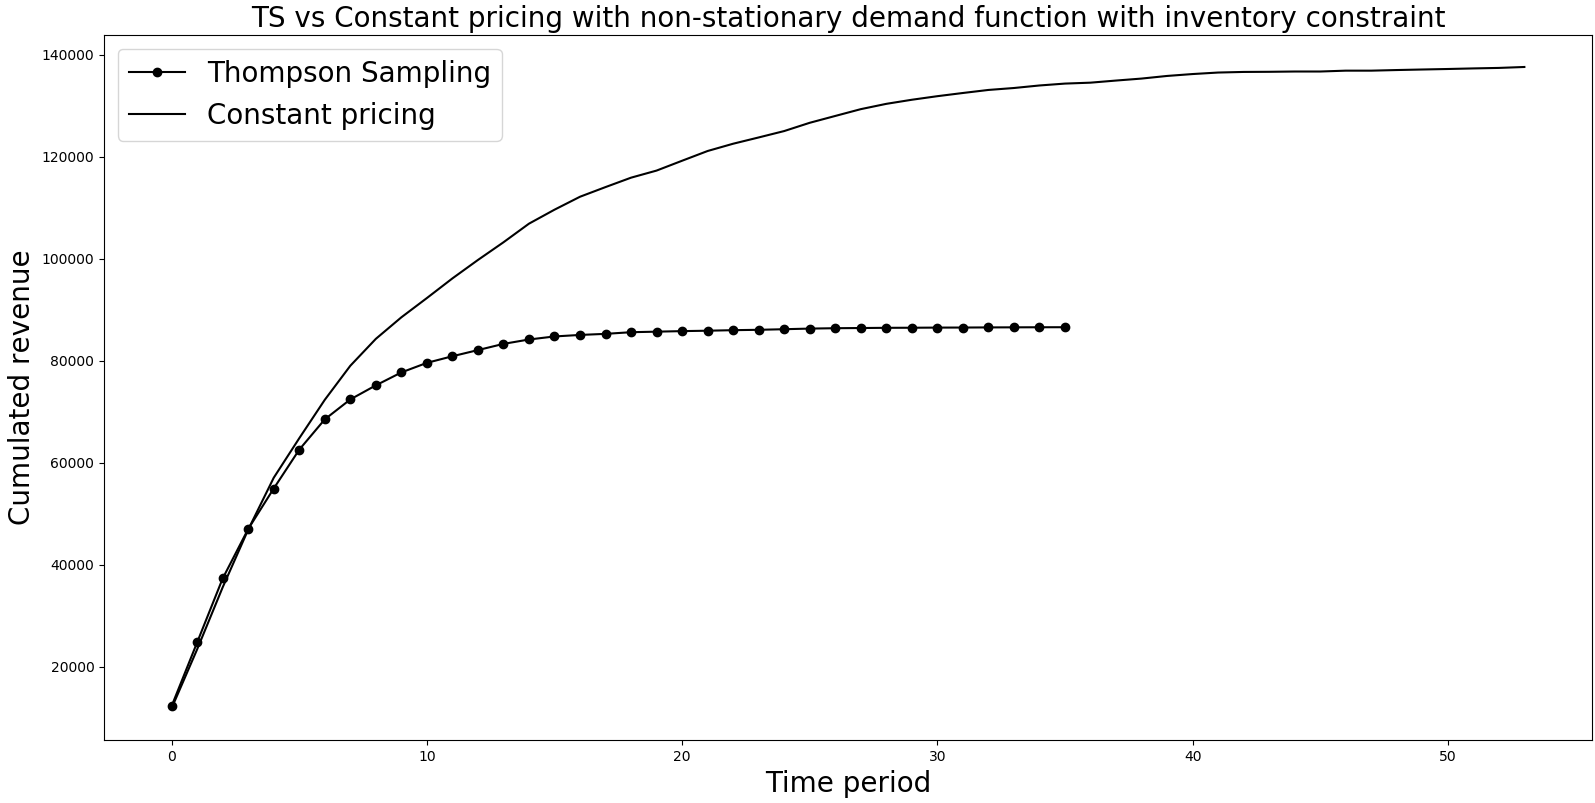
\includegraphics[width=1.03\textwidth]{4.png}
	\caption{\label{fig:five}Cumulated revenue of TS and constant pricing with inventory constraints}
\end{figure}
\newline
As seen in Figure \ref{fig:five}, Thompson sampling clears the inventory much quicker than the constant pricing model. However, the amount of revenue generated by Thompson sampling is significantly lower. The Thompson sampling algorithm increases revenue by lowering prices which will lead to an increase in demand since the products' demand is elastic. This is not reflected in Figure \ref{fig:five} and we believe the reason may be due to the fact that we are simply considering too many time periods and most of the products have already run out of inventory. In other words, before Thompson sampling terminated at around time period = 35, many products were actually already sold out from time period = 20 and there were only a couple of products there were still in stock.
\newline
\newline
If we cut off the plots at time period = 15, the constant pricing model earned 30.9\% more revenue than Thompson sampling but incurred 45.3\% more costs. It also sold 8.5\% less products than Thompson sampling but still managed to record 29.6\% more profits where profits = revenue - costs. Thus, the decrease in prices is not compensated by the increase in demand as there is simply insufficient stock to meet the market's demand. This further reinforces our belief that the seller should be able to meet the market's demand in each time period. It may be difficult to observe from Figure \ref{fig:five} but between the second and fourth points, the revenue by Thompson sampling is actually greater than the revenue by the constant pricing model and it closely resembles the plot in Figure \ref{fig:four}. After the fourth point, the plot of Thompson sampling starts to taper off. This is due to inventory running out and thus the observed demand for most products is 0. It may thus be more effective if we considered a shorter selling season with less time periods where we do not have to worry about products running out of inventory which leads us to the next subsection.

\subsubsection{Dynamic vs Constant pricing without constraint}
In this subsection, we do not impose any constraint and simply implement the algorithm proposed by the authors on the real dataset.
\begin{figure}[h]
	\centering
	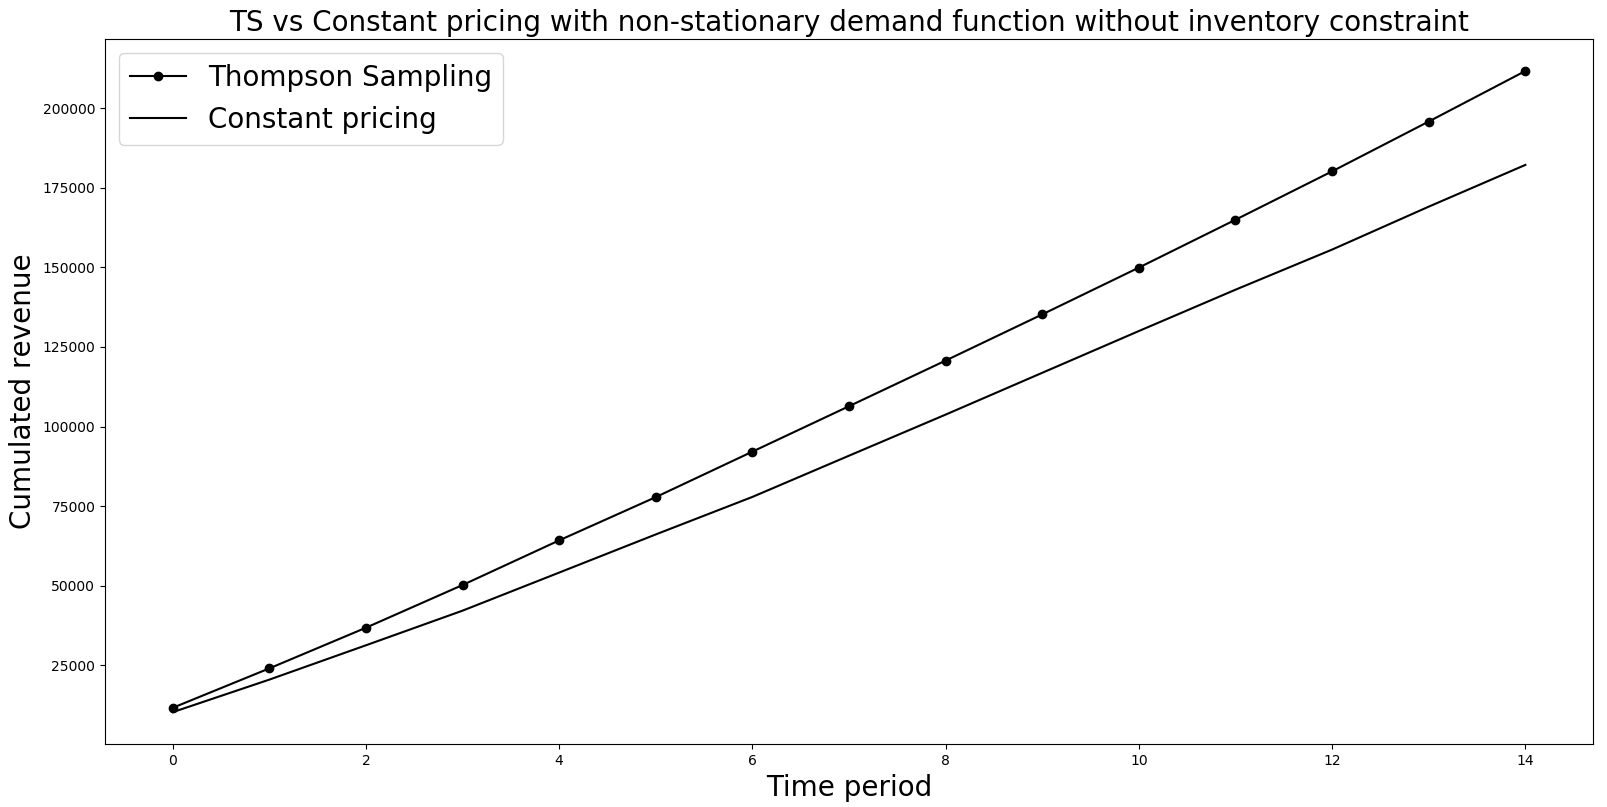
\includegraphics[width=1.03\textwidth]{512.png}
	\caption{\label{fig:four}Comparing cumulated revenue between TS and constant pricing without inventory constraints}
\end{figure}
\newline
Since we do not impose any inventory constraint, it is assumed that the seller has sufficient stock to satisfy demand in each time period. Just as in the previous subsection, in each successive time period, the price of products fall gradually while demand increases steadily. As the products are elastic in demand, the decrease in prices leads to a larger increase in demand which results in higher revenue.
\newline
\newline
By the end of the horizon, Thompson sampling earned 14.8\% more revenue than the constant pricing model and also sold 65.8\% more products. If we had 1500 of each product in inventory at the beginning of the selling season, we can also analyse the amount of inventory cleared. In most real world situations, products may no longer be sold after the selling season is over and there is a cost incurred by the seller for not being able to sell it. We can assign a cost to each product and investigate the total costs for each model. By setting cost $= 0.5  p_{i,0}$ and taking into account the amount of products left over, Thompson sampling had incurred 9.5\% less costs than the constant pricing model. On the whole, Thompson sampling made 12.3\% less losses where loss = costs - revenue. We chose 1500 as our stock because through several runs and experiments, we know that the amount of stock cleared by Thompson sampling generally does not exceed 1500 for each product after 15 time periods since we want to prevent inventory constraint from being a reason for Thompson sampling's poor performance.
\newline
\newline
We can frame this problem as trying to clear excess inventory during a finite selling season (15 time periods) and the decrease in prices as coupons offered to customers. Even though the main objective is to clear inventory, we also want to ensure that we are able to minimise losses and maximise profits as much as possible. Thus, when assuming no inventory constraints (the seller is able to meet the market's demand in every time period) and the independence of products' elasticities, the dynamic pricing algorithm works better.

\subsection{Stationary demand function}
In this section, the demand function is chosen to be the one in (1).
\subsubsection{Dynamic vs Constant pricing with constraint}
\begin{figure}[h]
	\centering
	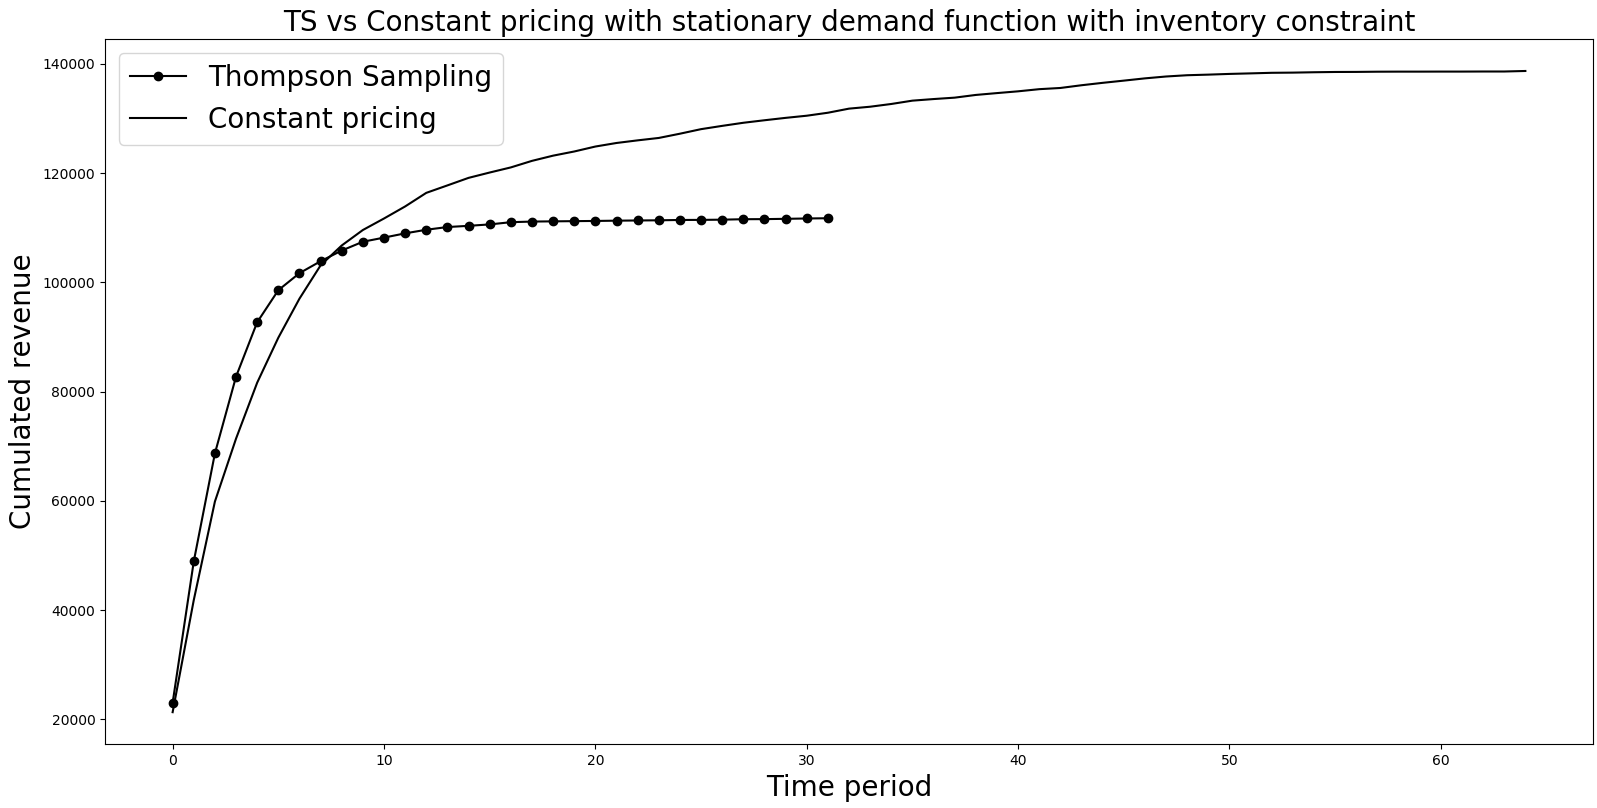
\includegraphics[width=1.03\textwidth]{3.png}
	\caption{\label{fig:3}Cumulated revenue of TS and constant pricing without inventory constrain}
\end{figure}
Here, we again set the amount of inventory to be 50 for each product in order to investigate the peformance of the algorithm under inventory constraints. Unfortunately, the algorithm's flaws that were exposed in section 5.1.1 also resurface here. In Figure \ref{fig:3}, we can see that the shape of the curve is very similar to the one seen in Figure \ref{fig:five}. The Thompson sampling algorithm again terminates much earlier than the constant pricing model which suggests that inventory is cleared much quicker. One interesting point to note is that in the early stages between points 1 to 8, we can see that the revenue increases at a much faster rate than in Figure \ref{fig:five} of the previous subsection. This suggests that Thompson sampling performs better when the demand function is stationary.
\newline
\newline
If we cut off the plots at time period = 15, the revenue earned by the constant pricing model is 13.1\% more than the revenue earned by the modified Thompson sampling algorithm. In terms of costs, Thompson sampling actually incurred 84.3\% less costs. If we define loss = costs - revenue, the constant pricing model recorded 7.9\% more profits. This is also observed in section 5.1.1 where Thompson sampling incurred less costs, earned less revenue and recorded less profits. We believe this is again due to the consideration of too many time periods since Thompson sampling lowers prices to stimulate more market demand. This would not work as there is not enough stock to meet the increase in market demand and so observed demand for products out of stock is 0. We next consider a shorter selling season with less time periods to investigate if shorter selling seasons would help to mitigate the problem.
\newpage
\subsubsection{Dynamic vs Constant pricing without constraint}
Similar to what was done in the non-stationary setting, we remove the inventory constraint and implement the algorithm on the real dataset with a stationary demand function.
\begin{figure}[h]
	\centering
	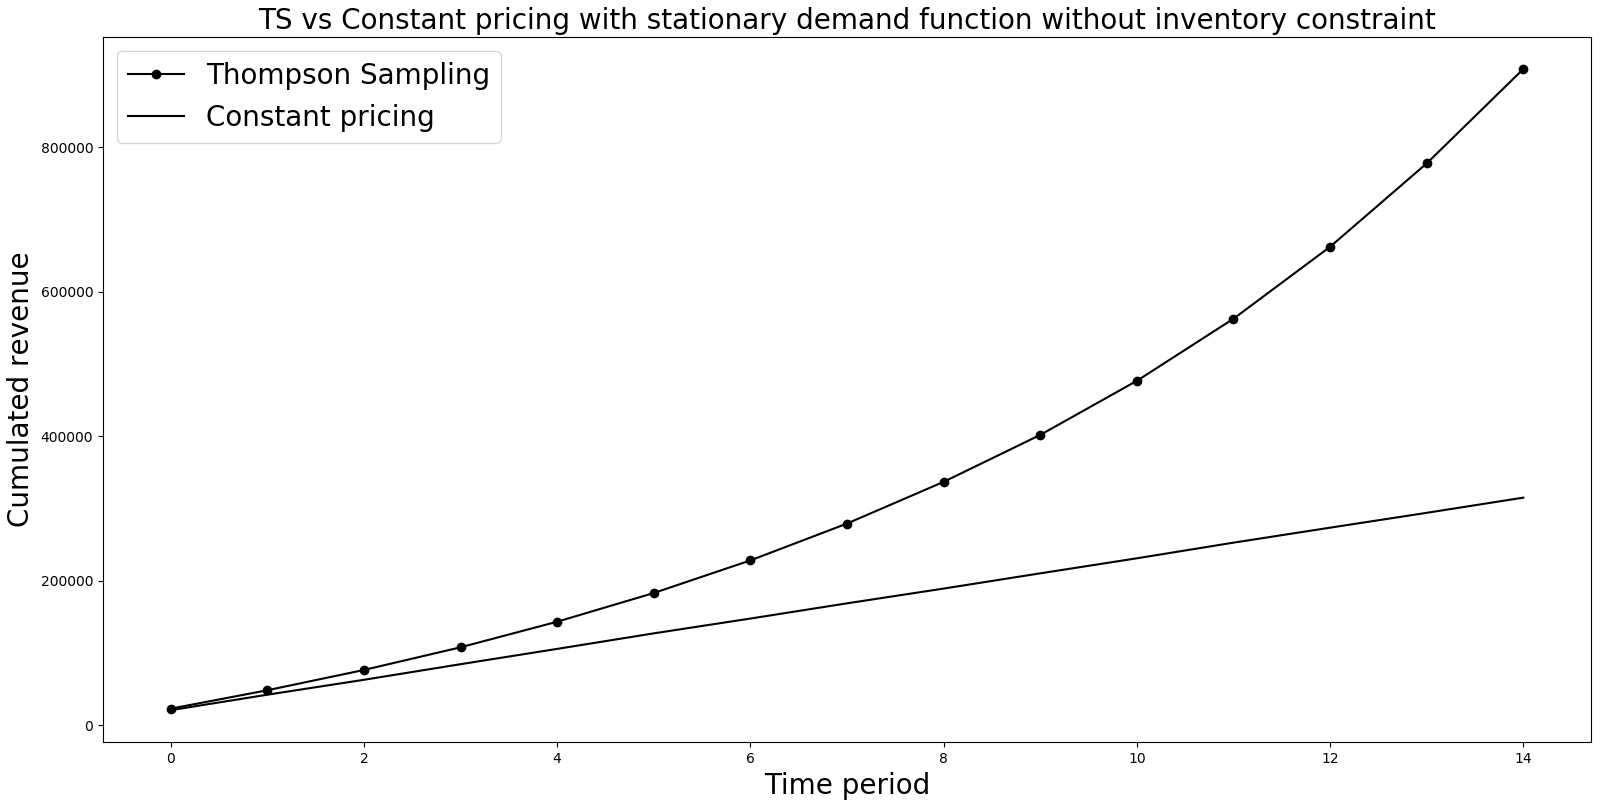
\includegraphics[width=1.03\textwidth]{522.png}
	\caption{\label{fig:1}Cumulated revenue of TS and constant pricing without inventory constraint}
\end{figure}
\newline
In this case, we see that Thompson sampling outperforms the constant pricing model. Since we removed the inventory constraint, it means that when Thompson sampling reduces prices to stimulate demand, the market demand is always met. This means that since the products have elastic demand in our initialisation, the decrease in prices leads to a larger increase in demand which results in more revenue.
\newline
\newline
Here, we set our inventory to be 10000 because we know that through several runs and experiments, the maximum amount of stock Thompson sampling would clear for a product will not exceed 10000 in 15 time periods and this would help to ensure that inventory constraint is not a problem in this setting. We cannot set it to be 1500 as in section 5.1.2 because Thompson sampling somehow sells more products under the stationary demand function. Setting our inventory to be 1500 would inadvertently reproduce the plot in Figure \ref{fig:3} where the seller runs out of stock. This is also why the cumulated revenue throughout section 5.2 is greater than the figures observed in section 5.1. The larger amount of products sold here also possibly explains why the Thompson sampling revenue in Figure \ref{fig:1} is growing at a much larger rate than in Figure \ref{fig:3}.
\newline
\newline
In terms of numbers, Thompson sampling had accumulated 65.3\% more revenue, incurred 7.7\% less costs and on the whole recorded 11.8\% less losses than the constant pricing model where loss = costs - revenue. This is consistent with our observations in section 5.1.2 since the seller can now meet the increasing market demand in each time period with the inventory constraint removed.


\subsection{Conclusion of second approach}
The Thompson sampling algorithm proposed by Ganti, Sustik, Tran \& Seaman (2018) works mostly well in both stationary and non-stationary settings assuming that the seller is able to meet the market's demand in every time period. The effectiveness of the algorithm is further amplified in the stationary case. It mostly outperforms the constant pricing model especially when there are no inventory constraints or when the selling season is short enough for inventory constraint to become a problem. Some possible extensions would be to compare this Thompson sampling algorithm to other algorithms adapted for infinite arms such as the confidence bound target (CBT) algorithm proposed by Chan \& Hy (2018)  or the UCB-F algorithm proposed by Wang, Audibert \& Munos (2009).

%\newpage
\section{Conclusion and future direction}
In this paper, we explored the algorithm known as Thompson sampling in various settings. We compared its performance to other well-known algorithms such as UCB in the MAB problem using a MNL demand function and the constant price elasticity function with both synthetic data and real data. We observed that Thompson sampling greatly outperformed greedy algorithms and to a smaller extent, UCB algorithms which are considered to be more commonly utilised. 
\newline
\newline
We then implemented a dynamic pricing algorithm using Thompson sampling proposed by Ganti, Sustik, Tran \& Seaman (2018) on a real dataset which consisted of sales data of children's books. In this approach, instead of the MNL model, we used a modified constant elasticity model as the demand function. We compared its performance to a constant pricing model in two different settings: with a non-stationary demand function and with a stationary demand function. For each of these settings, we further considered additional constraints, namely with inventory constraint and without inventory constraint. The results in both stationary and non-stationary settings were fairly similar so we will speak about both at the same time and highlight interesting points whenever necessary. 
\newline
\newline
In the setting without inventory constraint, Thompson sampling easily outperforms the constant pricing algorithm. It achieves higher revenue at less cost and is able to sell more products which led to larger profits than the constant pricing algorithm. In the setting with inventory constraints, we set the observed demand of products with depleted stock to be 0. From our observations, the constant pricing model outperforms Thompson sampling and it tapers off much later. This is because Thompson sampling sold more goods at a faster rate than the constant pricing model. Thus, the decrease in product prices by Thompson sampling is not being sufficiently compensated by the increase in demand as there is simply no stock left. Therefore, a required assumption of the dynamic pricing algorithm with Thompson sampling is that either the seller must be able to meet customers' demand in the entire horizon or the selling season should be shortened such as inventory constraint is not a concern.
\newline
\newline
As we saw in the second approach, the dynamic pricing algorithm with Thompson sampling fails when inventory constraints are introduced and only succeeds when the seller knows they can meet market demand during the selling season. In certain real world markets, this may not be a very flexible assumption since demand may change overtime due to external events. A seller might be in the middle of the selling season when he realises his supply is insufficient due to changes in the market. He will then have to cease Thompson sampling or risk incurring losses. It may thus be worthwhile to investigate extending this dynamic pricing algorithm with Thompson sampling to be more robust against inventory constraints. A possible direction would be to incorporate inventory constraints more elegantly instead of setting observed demand to be simply 0. A good resource to start with would be Ferreira, Simchi-Levi \& Wang (2017)'s paper where they investigate different products requiring different kinds of resources in detail.
\newpage

\begin{thebibliography}{9}
	\bibitem{nano3}
	https://www.statista.com/statistics/534123/e-commerce-share-of-retail-sales-worldwide/
	
	\bibitem{CK}
	https://milled.com/CalvinKlein/final-hours-take-40-off-every-100-spent-Q2RTJAp7mfdfwq3I
	
	\bibitem{anderson}
	Anderson, Jaimovich, Simester. 2015. Price stickiness: Empirical evidence of the menu cost channel. \emph{Review of Economics and Statistics} 97(4):813–826.
	
	\bibitem{1}
	Araman, V. F., R. Caldentey. 2009. Dynamic pricing for nonperishable products with demand learning.
	\emph{Operations Research} 57(5) 1169-1188.
	
	\bibitem{1a}
	Aviv, Pazgal. 2005. A partially observed markov decision process for dynamic
	pricing. \emph{Management Science} 51(9) 1400–1416.
	
	\bibitem{bada}
	Badanidiyuru, A., R. Kleinberg, A. Slivkins. 2013. Bandits with knapsacks. \emph{IEEE 54th Annual Symposium on Foundations of Computer Science (FOCS).} 207-216.	
	
	\bibitem{brod}
	Broder, Rusmevichientong. 2012. Dynamic pricing under a general parametric choice model. \emph{Operations Research} 60(4) 965-980.
	
	\bibitem{bub}
	Bubeck, S., N. Cesa-Bianchi. 2012. Regret analysis of stochastic and nonstochastic multi-armed bandit problems. \emph{Foundations and Trends in Machine Learning} 5(1) 1-122.
	
	\bibitem{thomp}
	Chapelle,  Li. 2011. An Empirical Evaluation of Thompson Sampling. NIPS. 
	
	\bibitem{2}
	Farias, V., B. Van Roy. 2010. Dynamic pricing with a prior on market response. \emph{Operations Research} 58(1) 16-29.
	
	\bibitem{inventory}
	Ferreira, Simchi-Levi, Wang. 2017. Online Network Revenue Management Using Thompson Sampling. \emph{Operations Research}
	
	\bibitem{main}
	Ganti, Sustik, Tran, Seaman. 2018. Thompson Sampling for Dynamic Pricing. 
	
	\bibitem{cbt}
	Hock, Hu. 2018. Infinite Arms Bandit: Optimality via Confidence Bounds.
	
	\bibitem{ucbf}
	Wang, Audibert, Munos. 2009. Algorithms for Infinitely Many-Armed Bandits.
\end{thebibliography}



\end{document}